% Created 2023-05-10 Wed 12:04
% Intended LaTeX compiler: pdflatex
\documentclass[aspectratio=169,t]{beamer}
\usepackage[utf8]{inputenc}
\usepackage[T1]{fontenc}
\usepackage{graphicx}
\usepackage{longtable}
\usepackage{wrapfig}
\usepackage{rotating}
\usepackage[normalem]{ulem}
\usepackage{amsmath}
\usepackage{amssymb}
\usepackage{capt-of}
\usepackage{hyperref}
\usepackage{listings}
\setbeamerfont{caption}{size=\footnotesize}
\usepackage{animate}
\usepackage{mathtools}
\DeclarePairedDelimiter\abs{\lvert}{\rvert} % ABS: abs{}
\usetheme{focus}
\author{Samuel J Monson}
\date{2023-03-07}
\title{Complex and Hypercomplex \\ Iterative Methods}
\definecolor{main}{HTML}{93361f}
\definecolor{background}{HTML}{D0D0D0}
\setmathfont{Fira Math}
\setmathfont{DejaVu Math TeX Gyre}[range=\vysmwhtcircle]
\setmonofont{Hack}
\hypersetup{
 pdfauthor={Samuel J Monson},
 pdftitle={Complex and Hypercomplex \\ Iterative Methods},
 pdfkeywords={},
 pdfsubject={},
 pdfcreator={Emacs 30.0.50 (Org mode 9.6.1)}, 
 pdflang={English}}
\begin{document}

\begin{frame}
\maketitle
\end{frame}
\begin{frame}[label={sec:org197d34e}]{Iteration}
\begin{definition}[Function Iteration]\label{sec:org9c674fc}
\(f^0 := \symbf{I}\)

\(f^{k+1} := f \circ f^k\)
\end{definition}

\begin{exampleblock}{Example}\label{sec:orgc1b4f0d}
Given \(f(x) = x + 1\),

\begin{align*}
    \only<2->{f^0(x) & = x} \\
    \only<3->{f^1(x) & = x + 1} \\
    \only<4->{f^2(x) & = (x + 1) + 1}
\end{align*}
\end{exampleblock}
\end{frame}

\begin{frame}[label={sec:org9e152a1}]{Complex Dynamics}
\begin{columns}
\begin{column}{0.5\columnwidth}
\begin{definition}[Dynamical System]\label{sec:org56dd4b0}
A system that enacts rules on a set of variables to produce a state.
\end{definition}
\end{column}

\begin{column}{0.5\columnwidth}
\begin{definition}[Complex Dynamics]\label{sec:orgbf27de6}
The study of \uline{Dynamical Systems} defined by complex iterative functions.
\end{definition}
\end{column}
\end{columns}
\end{frame}


\begin{frame}[label={sec:org4d7d28f}]{Complex Numbers}
\begin{definition}[Complex Numbers]\label{sec:org4596063}
\(\symbf{i}^2 = -1\)

\(\{a + b \symbf{i} : a,b \in \symbb{R} \} \in \symbb{C}\)
\end{definition}
\end{frame}

\begin{frame}[label={sec:org4ab5998}]{Complex Iteration}
\begin{columns}
\begin{column}{0.5\columnwidth}
\begin{block}{Rules}
\(f(z) = z^2\)

\(z_0 = \frac{1}{\sqrt{2}} + \frac{1}{\sqrt{2}} \symbf{i}\)
\end{block}

\begin{itemize}[<+->]
\item \(f^0(z) = \frac{1}{\sqrt{2}} + \frac{1}{\sqrt{2}} \symbf{i}\)
\item \(f^1(z) \only<2>{= \left( \frac{1}{\sqrt{2}} + \frac{1}{\sqrt{2}} \symbf{i} \right)^2 = \left( \frac{1}{\sqrt{2}} \right)^2 - \left(\frac{1}{\sqrt{2}} + \frac{1}{\sqrt{2}}\right)^2 + \left(\frac{1}{\sqrt{2}} + \frac{1}{\sqrt{2}}\right)^2 \symbf{i}} = \symbf{i}\)
\item \(f^2(z) = -1\)
\item \(f^3(z) = 1\)
\end{itemize}
\end{column}

\begin{column}{0.5\columnwidth}
\begin{center}
\includegraphics<1>[width=.9\linewidth]{Figs/exports/Iter_1-1.png}
\includegraphics<2>[width=.9\linewidth]{Figs/exports/Iter_1-2.png}
\includegraphics<3>[width=.9\linewidth]{Figs/exports/Iter_1-3.png}
\includegraphics<4>[width=.9\linewidth]{Figs/exports/Iter_1-4.png}
\end{center}
\end{column}
\end{columns}
\end{frame}

\begin{frame}[label={sec:org788f180}]{Complex Iteration}
\begin{columns}
\begin{column}{0.5\columnwidth}
\begin{block}{Rules}
\(f(z) = z^2 - \frac{1}{10} - \frac{1}{10} \symbf{i}\)

\(z_0 = \frac{1}{\sqrt{2}} + \frac{1}{\sqrt{2}} \symbf{i}\)
\end{block}

\begin{itemize}[<+->]
\item \(f^0(z) = \frac{1}{\sqrt{2}} + \frac{1}{\sqrt{2}} \symbf{i}\)
\item \(f^1(z) \only<2>{= -\frac{1}{10} + \left(1 - \frac{1}{10}\right)\symbf{i}} = -0.9 - 0.28\symbf{i}\)
\item \(f^2(z) = 0.6316+0.404\symbf{i}\)
\item \(f^3(z) \approx 0.13570256 + 0.4103328\symbf{i}\)
\end{itemize}
\end{column}

\begin{column}{0.5\columnwidth}
\begin{center}
\includegraphics<1>[width=.9\linewidth]{Figs/exports/Iter_2-1.png}
\includegraphics<2>[width=.9\linewidth]{Figs/exports/Iter_2-2.png}
\includegraphics<3>[width=.9\linewidth]{Figs/exports/Iter_2-3.png}
\includegraphics<4>[width=.9\linewidth]{Figs/exports/Iter_2-4.png}
\end{center}
\end{column}
\end{columns}
\end{frame}

\begin{frame}[label={sec:orgb5d6dae}]{Group Activity}
\(f(z) = z^2 + c\)

\begin{columns}
\begin{column}{0.5\columnwidth}
\begin{block}{Easier}
\(c = -0.2 + 0 \symbf{i}\)

\(z_0 = 0.5 + 0 \symbf{i}\)
\end{block}
\end{column}

\begin{column}{0.5\columnwidth}
\begin{block}{Harder}
\(c = -0.2 + 0.4 \symbf{i}\)

\(z_0 = 0.5 - 0.5 \symbf{i}\)
\end{block}
\end{column}
\end{columns}
\end{frame}

\begin{frame}[label={sec:org83b3505}]{Group Activity (Easier)}
\begin{columns}
\begin{column}{0.5\columnwidth}
\begin{block}{Rules}
\(f(z) = z^2 + c\)

\(c = -0.2 + 0 \symbf{i}\)

\(z_0 = 0.5 + 0 \symbf{i}\)
\end{block}

\begin{itemize}[<+->]
\item \(f^1(z) = 0.05\)
\item \(f^2(z) = -0.1975\)
\item \(f^3(z) = -0.16099375\)
\item \(f^4(z) = -0.1740810125\)
\end{itemize}
\end{column}

\begin{column}{0.5\columnwidth}
\begin{center}
\includegraphics<1>[width=.9\linewidth]{Figs/exports/Iter_3-1.png}
\includegraphics<2>[width=.9\linewidth]{Figs/exports/Iter_3-2.png}
\includegraphics<3>[width=.9\linewidth]{Figs/exports/Iter_3-3.png}
\includegraphics<4>[width=.9\linewidth]{Figs/exports/Iter_3-4.png}
\end{center}
\end{column}
\end{columns}
\end{frame}

\begin{frame}[label={sec:org9f46756}]{Group Activity (Harder)}
\begin{columns}
\begin{column}{0.5\columnwidth}
\begin{block}{Rules}
\(f(z) = z^2 + c\)

\(c = -0.2 + 0.4 \symbf{i}\)

\(z_0 = 0.5 - 0.5 \symbf{i}\)
\end{block}

\begin{itemize}[<+->]
\item \(f^1(z) = -0.2 - 0.1 \symbf{i}\)
\item \(f^2(z) = -0.17 + 0.44 \symbf{i}\)
\item \(f^3(z) = -0.3647 + 0.2504 \symbf{i}\)
\item \(f^4(z) = -0.12969407 + 0.21735824 \symbf{i}\)
\end{itemize}
\end{column}

\begin{column}{0.5\columnwidth}
\begin{center}
\includegraphics<1>[width=.9\linewidth]{Figs/exports/Iter_4-1.png}
\includegraphics<2>[width=.9\linewidth]{Figs/exports/Iter_4-2.png}
\includegraphics<3>[width=.9\linewidth]{Figs/exports/Iter_4-3.png}
\includegraphics<4>[width=.9\linewidth]{Figs/exports/Iter_4-4.png}
\end{center}
\end{column}
\end{columns}
\end{frame}

\begin{frame}[label={sec:orgf1f1b04},fragile]{Implementation}
 \begin{block}{Iteration}
\begin{lstlisting}[language=Python,firstnumber=1,numbers=left]
N = 128
B = 16
c = complex(-0.675, -0.112)
def iterate(z):
    for n in range(N):
        z = z*z + c
        if abs(z) > B: break
    return n
\end{lstlisting}
\end{block}
\end{frame}

\begin{frame}[label={sec:org05a310b}]{Iterative Fractals}
\begin{columns}
\begin{column}{0.55\columnwidth}
\begin{block}{Complex Juila Set Example}
Defined by iterative function in complex space

\begin{itemize}
\item \(f_c (z) = z^2 + c\)

\item \(\left\{ z_0 \in \symbb{C}: \abs{f^k_c \left(z_0 \right)} \in \symbb{C} \text{ as } k \to \infty\right\} \in K_c\)
\end{itemize}
\end{block}
\end{column}

\begin{column}{0.45\columnwidth}
\begin{center}
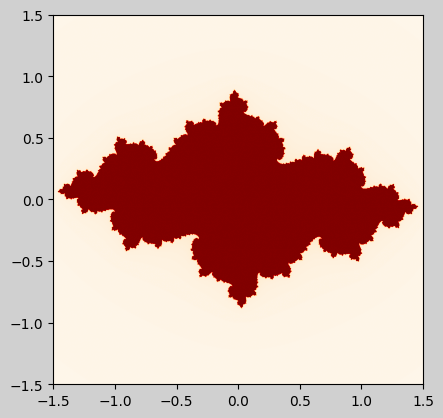
\includegraphics[width=0.95\textwidth]{./Figs/Fig_2.png}
\end{center}
\end{column}
\end{columns}
\end{frame}


\begin{frame}[label={sec:org165ee9e}]{Hypercomplex (Quaternions)}
\begin{definition}[Quaternion]\label{sec:org0ab27ed}
\(\symbf{i}^2 = \symbf{j}^2 = \symbf{k}^2 = \symbf{ijk} = -1\)

\(\left\{ d + a\symbf{i} + b\symbf{j} + c\symbf{k} : a,b,c,d \in \symbb{R} \right\} \in \symbb{H}\)
\end{definition}

\begin{columns}
\begin{column}{0.50\columnwidth}
\begin{itemize}[<+->]
\item \(\symbf{i}^2 = \symbf{ijk}\)
\begin{itemize}
\item \(\symbf{i}^{-1} \symbf{i}^2 = \symbf{i}^{-1} \symbf{ijk}\)
\item \(\symbf{i} = \symbf{jk}\)
\end{itemize}
\item \(\symbf{k}^2 = \symbf{ijk}\)
\begin{itemize}
\item \(\symbf{k}^2 \symbf{k}^{-1} = \symbf{ijk} \symbf{k}^{-1}\)
\item \(\symbf{k} = \symbf{ij}\)
\end{itemize}
\item \(\symbf{j} = \symbf{ki}\)
\end{itemize}
\end{column}

\begin{column}{0.50\columnwidth}
\begin{itemize}[<+->]
\item \(\symbf{i} = \symbf{jk}\)
\begin{itemize}
\item \(\symbf{ji} = \symbf{jjk}\)
\item \(\symbf{ji} = \symbf{j}^2 \symbf{k}\)
\item \(\symbf{ji} = -\symbf{k}\)
\item \(-\symbf{k} = \symbf{ji}\)
\end{itemize}
\item \(-\symbf{i} = \symbf{kj}\)
\item \(-\symbf{j} = \symbf{ik}\)
\end{itemize}
\end{column}
\end{columns}
\end{frame}

\begin{frame}[label={sec:org14292ca}]{Hypercomplex (Quaternions)}
\(\symbf{i}^2 = \symbf{j}^2 = \symbf{k}^2 = \symbf{ijk} = -1\)

\(p = d + a\symbf{i} + b\symbf{j} + c\symbf{k}\)

\(q = w + x\symbf{i} + y\symbf{j} + z\symbf{k}\)

\begin{align*}
    p \times q & = dw + dx\symbf{i} + dy\symbf{j} + dz\symbf{k} \\
    & + aw\symbf{i} + ax\symbf{i}^2 + ay\symbf{ij} + az\symbf{ik} \\
    & + bw\symbf{j} + bx\symbf{ji} + by\symbf{j}^2 + bz\symbf{jk} \\
    & + cw\symbf{k} + cx\symbf{ki} + cy\symbf{kj} + cz\symbf{k}^2
\end{align*}
\end{frame}

\begin{frame}[label={sec:orgc3606f6}]{Hypercomplex (Quaternions)}
\end{frame}

\begin{frame}[label={sec:orgd1b4a95}]{Group Activity}
\(f(z) = z^2 + q\)

\begin{columns}
\begin{column}{0.5\columnwidth}
\begin{block}{Easier}
\(q = -0.2 + 0.4\symbf{i} + 0\symbf{j} + 0\symbf{k}\)

\(z_0 = 0.5 - 0.5\symbf{i} + 0\symbf{j} + 0\symbf{k}\)
\end{block}
\end{column}

\begin{column}{0.5\columnwidth}
\begin{block}{Harder}
\(q = -0.2 + 0.4\symbf{i} + 0\symbf{j} + 0\symbf{k}\)

\(z_0 = 0.5 - 0.5\symbf{i} + 0\symbf{j} + 0\symbf{k}\)
\end{block}
\end{column}
\end{columns}
\end{frame}

\begin{frame}[label={sec:org96ffbc5},fragile]{Implementation}
 \begin{block}{Quaternion Multiplication}
\begin{lstlisting}[language=Python,firstnumber=1,numbers=left]
def qMult(p, q):
    r = Quat(
        p.r*q.r – p.i*q.i – p.j*q.j - p.k*q.k,
        p.r*q.i + p.i*q.r + p.j*q.k - p.k*q.j,
        p.r*q.j – p.i*q.k + p.j*q.r + p.j*q.i,
        p.r*q.k + p.i*q.j – p.j*q.i + p.k*q.r
    )
    return r
\end{lstlisting}
\end{block}
\end{frame}

\begin{frame}[label={sec:org77b3ca5},fragile]{Implementation}
 \begin{block}{Quaternion Square}
\begin{lstlisting}[language=Python,firstnumber=1,numbers=left]
def qSquare(q):
    r = Quat(
        q.r*q.r – q.i*q.i – q.j*q.j - q.k*q.k,
        2*q.r*q.i,
        2*q.r*q.j,
        2*q.r*q.k
    )
    return r
\end{lstlisting}
\end{block}
\end{frame}

\begin{frame}[label={sec:org397cf0d},fragile]{Implementation}
 \begin{block}{Quaternion Add}
\begin{lstlisting}[language=Python,firstnumber=1,numbers=left]
def qAdd(p, q):
    r = Quat(
        p.r + q.r,
        p.i + q.i,
        p.j + q.j,
        p.k + q.k
    )
    return r
\end{lstlisting}
\end{block}
\end{frame}

\begin{frame}[label={sec:org375b5fd},fragile]{Implementation}
 \begin{block}{Iteration}
\begin{lstlisting}[language=Python,firstnumber=1,numbers=left]
N = 12
B = 16
c = Quat(-0.2, 0.4, -0.4, -0.4)
def iterate(z):
    for n in range(N):
        z = z*z + c
        if abs(z) > B: break
    return n
\end{lstlisting}
\end{block}
\end{frame}

\begin{frame}[label={sec:orgc997dfb}]{Raytracing}
\end{frame}

\begin{frame}[label={sec:org7aa7ee5}]{Ray Marching}
\end{frame}

\begin{frame}[label={sec:org96a6846}]{Normal Estimation}
\end{frame}

\begin{frame}[label={sec:org5d951ac}]{Hypercomplex Iterative Fractals}
\begin{columns}
\begin{column}{0.55\columnwidth}
\begin{block}{Hypercomplex Juila Set Example}
\begin{itemize}
\item Defined by iterative function in 4D Quaternion space
\end{itemize}
\end{block}
\end{column}

\begin{column}{0.45\columnwidth}
\begin{center}
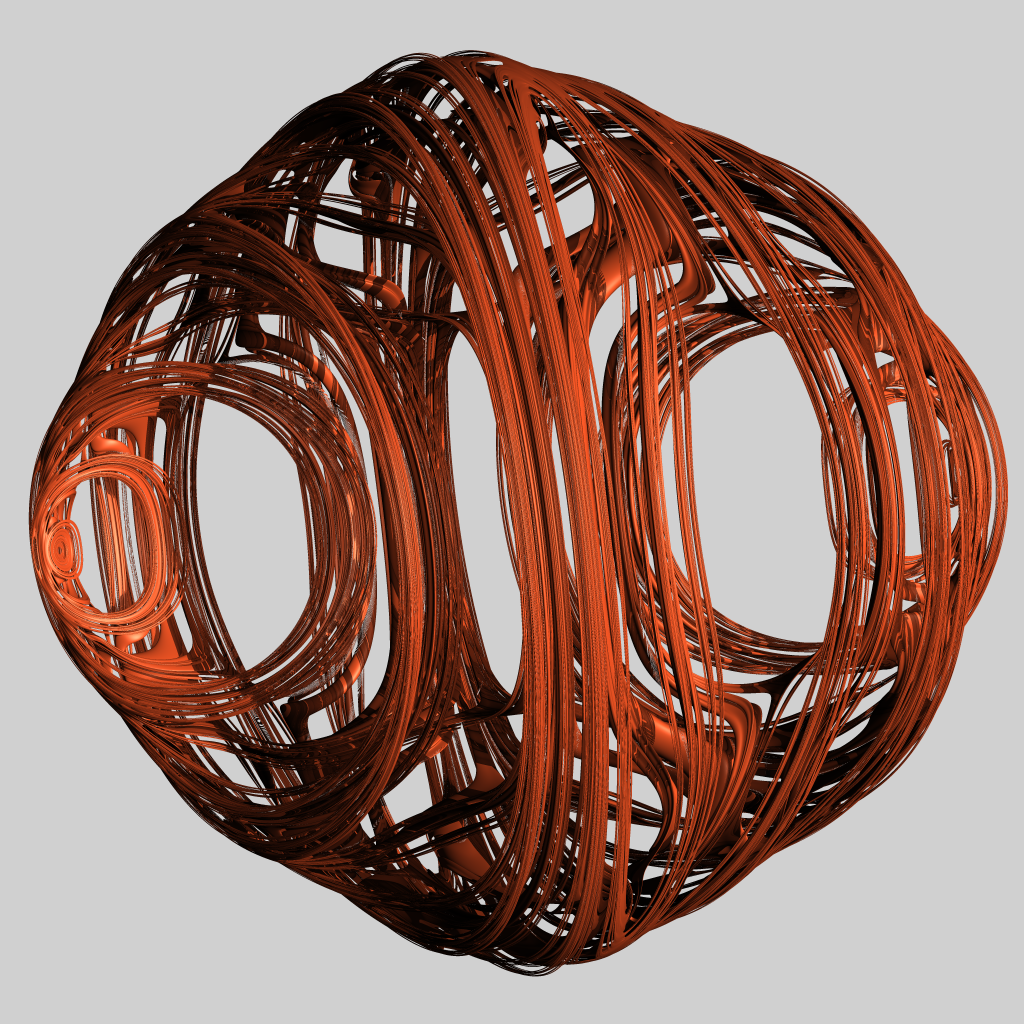
\includegraphics[width=0.95\textwidth]{./Figs/Fig_1v2.png}
\end{center}
\end{column}
\end{columns}
\end{frame}

\begin{frame}[label={sec:orga157e88}]{Conclusion}
%\animategraphics[autoplay,interpolate,height=4.0cm,loop]{7}{Figs/Test/}{1}{14}
\end{frame}

\begin{frame}[allowframebreaks,label=]{References}
\nocite{*}
\bibliography{sources}
\bibliographystyle{alpha}
\end{frame}
\end{document}